\chapter{Influence of fluid dynamics of the system on the extracted power}

\section{Introduction}

Galloping occurs as a result of the pressure difference created due to the relative distance between the shear layers and the respective walls of the cross section, at the top and bottom sides of the body. As discussed in section \ref{subsec:c_y and shear layers}, the instantaneous induced angle makes one of the separated shear layers closer to the wall creating a low pressure region. This pressure difference results in a traverse forcing (normal to the direction of the flow) which becomes in phase with the transverse velocity and sustains galloping. 

From equation \ref{eqn:power_alt} discussed in section \ref{subsec:ave_pow} it is clear that the power transferred from fluid to the body is a function of the induced forcing $F_y$ and the transverse velocity $\dot{y}$. The sign of the average power represents the direction of power transfer where the $+$ ve sign represents the power transfer from fluid to the body and $-$ ve being power transferring from body to the fluid. 

Thus, then  according to equation \ref{eqn:power_alt} it can be deduced that if there is a scenario where both high induced forcing and high transverse velocities are present, higher power output could be achieved. This brings to the analysis of the $C_y$ vs. $\theta$ curve. \citet{Luo1994}, showed that the afterbody of the cross section has a direct impact on $C_y$ vs. $\theta$ curve. One interesting observation of this study was that delaying the shear layer re-attachment results in higher peak induced force coefficient $C_y$ occurring at high induced angles (high transverse velocities).    

Therefore, it could be hypothesised that a higher power transfer could be obtained by delaying the shear layer re-attachment. 

Here, the influence of shear layer and its reattachment on the mean power is studied by introducing a cross section which is a hybrid of a square and a triangle. The cross section is transformed gradually by manipulating the ratio of two length scales.

The stationary forcing data are presented for each cross section followed by the QSS power curves. Based on the QSS power data, an optimum cross section for power extraction is identified. As a negative region on some $C_y$ vs. $\theta$ curves were observed, the underpinning reason for this region was investigated through an analysis of the surface pressure and flow velocity data. The results and discussion of this analysis are presented. Following this, a comparison is made between QSS and DNS mean power at on the cross section which provides an optimum mean power.       

A final summary is presented explaining the influence of the behaviour of the shear layer on mean power output and the preliminary design considerations to optimise the fluid mechanics to obtain an optimum power output. 

\section{Influence of the shear layers}

In a typical cross section which sustains galloping, the induced lift \cy\ increases with increasing induced angle $\theta$ until it reaches a maximum value of \cy where the shear layer re attachment occurs. The lift force then decreases as $\theta$ is further increased. The underlying mechanism for this behaviour is discussed in detail in section \ref{subsec:c_y and shear layers}.   

\subsection*{Selection of the cross section}

\begin{figure}
\setlength{\unitlength}{\textwidth}

  \begin{picture}(1,0.23)(0,0.74)
    
  \put(0.2,0.76){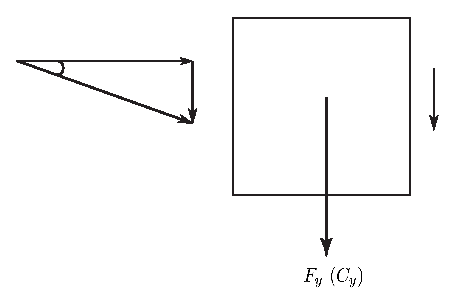
\includegraphics[width=0.5\unitlength]{../FnP/gnuplot/setup-1.eps}}         
      
      
   
 	\put(0.315,0.93){$U$}
 	\put(0.3,0.84){$U_i$}
    \put(0.42,0.88){$\dot{y}$}
    \put(0.28,0.895){ $\theta$}
    \put(0.7,0.87){\small $(+)$}
      	

 	
 	 

     

  \end{picture}

 \caption{Induced angle of attack on the square prism due to the resultant of free-stream velocity of the fluid and transverse velocity of the body.}
    \label{fig:setup_1}
\end{figure}

The cross section selected to test the shear layer influence on power was a hybrid cross section of a square and a triangle or in other words a pentagon which is illustrated in figure \ref{fig:hybrid_section}. This was produced by systematically tapering off the trailing edges of the top and bottom sides of the square cross section. The $\ratio$ was changed gradually from 1 to zero at increments of 0.25 where 1 being the square cross section and 0 being an isosceles triangle. This type of a cross section was selected because after analysing the shear layer behaviour of a galloping body it was found out that it is crucial to have the afterbody and the shear layer close to the body. And therefore the presence of the horizontal part of the top and bottom sides of the cross section. Rectangular cross sections are not very suitable as it may have a earlier shear layer re-attachment \citet{Paidoussis2010}. Another option was to use trapeziums as \citet{Luo1994}. However, the initial shear layers are quite far away and thus, maybe difficult to initialise galloping. The main focus was to study influence of shear layer behaviour on galloping, and thus the current hybrid cross section was used to study this behaviour by systematically delaying the shear layer reattachment of the initial square cross section. 

\section{Static body results}
\label{sec:cross-sec-Static body results}
\begin{table}[ht]

\begin{center}
\setlength{\unitlength}{\textwidth}

\begin{tabular}{c c c c c} % centered columns (4 columns)
\hline\hline %inserts double horizontal lines
\\[0.2ex]
Case & $a_1$ & $a_3$ & $a_5$ & $a_7$ \\ [0.8ex] % inserts table 
%heading
\hline 
\\[0.8ex]% inserts single horizontal line
Re=200 & 2.32 & 197.8 & 4301.7 & 30311.9 \\[0.8ex]% inserting body of the table
Re=22300 & 2.69 & 168 & 1670 & 59900 \\ [1ex] % [1ex] adds vertical space
\hline %inserts single line
\end{tabular}

\caption{Coefficient values used in the 7th order interpolation polynomial for high ($Re=22300$) and low ($Re=200$) Reynolds numbers. These data are used as input data to calculate the right-hand side of Eq. \ref{final_equation_motion} throughout this study.}
 
\label{table:cy-coefficients} % is used to refer this table in the text
\end{center}
\end{table}



Stationary time averaged $C_y$ results were obtained for cross sections where $\ratio=1,0.75,0.5,0.25$ and $0$ using DNS at $\reynoldsnumber=200$. Where $\ratio=1$ being the square and $\ratio=0$ being an isosceles  triangle. Table \ref{table:cy-coefficients-hybrid} shows the coefficients of the $7^{th}$ order curve fitting for each cross section. In order to achieve a better fit, piecewise interpolation using multiple $7th$ order polynomials were incorporated for a single cross section. During the curve fitting process more importance was given for accurately fitting  the positive portion of the $C_{y}$ curve, as the power transfer from the fluid to the body occur in this region. 

\begin{figure}
  \setlength{\unitlength}{\textwidth}

  \begin{picture}(1,0.75)(0,0)
    % % %90
      % % % Parkinson Data 
      \put(0.035,0.5){\includegraphics[width=0.5\unitlength]{./FnP/lift_curve_sq.eps}}
      \put(0.495,0.5){\includegraphics[width=0.5\unitlength]{./FnP/lift_curve_075.eps}}
      \put(0.035,0.27){\includegraphics[width=0.5\unitlength]{./FnP/lift_curve_05.eps}}
      \put(0.495,0.27){\includegraphics[width=0.5\unitlength]{./FnP/lift_curve_025.eps}}
      \put(0.3,0.0){\includegraphics[width=0.5\unitlength]{./FnP/lift_curve_tri.eps}}
      
      
   
      
      
%      \put(0.23,0.00){ $\displaystyle\frac{c}{\rho\mathcal{A}U}$}
%      \put(0.73,0.00){ $\displaystyle\frac{c}{\rho\mathcal{A}U}$}

      \put(0.3,0.26){$\theta$}
      \put(0.76,0.26){$\theta$}
      \put(0.56,-0.01){$\theta$}
      
      \put(0.01,0.405){$\displaystyle C_y$}
       \put(0.01,0.65){$\displaystyle C_y$}
      \put(0.3,0.14){$\displaystyle C_y$}
      
      \put(0.106,0.705){\small(a)}
      \put(0.565,0.705){\small(b)}
      \put(0.106,0.475){\small(c)}
      \put(0.565,0.475){\small(d)}
      \put(0.37,0.207){\small(e)}
      

  \end{picture}

  \caption{Induced lift coefficient $C_y$ at different angles for selected cross sections. Data presented for cross sections, (a) square, (b) $\ratio=0.75$, (c) $\ratio=0.5$, (d) $\ratio=0.25$ and (e) triangle.}
  \label{fig:lift_curves}
\end{figure} 

The $C_y$ vs. $\theta$ curves in figure \ref{fig:lift_curves-hybrid} shows that the peak value of \cy\ shifts to the right as $\ratio$ is increased, hence, the peak \cy\ occurs at high induced angles.  These data agree with \citet{Luo1994} where the peak of the maximum \cy\ value was shifted to higher induced angles when reattachment was delayed. As $\theta$ is proportional to the transverse velocity of the body $\tan{\theta}=\frac{\dot{y}}{U}$, the peak value of \cy\ occurs at high induced velocities as \ratio\ is decreased. A negative region of $C_y$ vs. $\theta$ curves on cross sections where $\ratio\geq0.25$. Here, initially \cy\ decreases as $\theta$ is increased and the increases after reaching a minimum. The presence of this negative portion is an indication of unfavourable power transfer, .i.e. power transferred from body to the fluid as the direction of the force and velocity vectors are out of phase. This will be further discussed in the upcoming sections of this chapter.    

 
 
 \section{QSS Mean power output}
 \label{sec:cross-sec-qss-mean power}
 
 % !TeX spellcheck = en_GB
\begin{figure}[!htb]
  \setlength{\unitlength}{\textwidth}

        \begin{picture}(1,0.4)(-0.02,0)

 
      
      \put(0.08,0.02){\includegraphics[width=0.75\unitlength]{./chapter-cross-sections/fnp/mean_power_hyb.eps}}

      \put(0.46,0.00){\massdamp}
      
      
     
       \put(0.03,0.235){$\displaystyle\frac{P_{m}}{\rho \mathcal{A}U^3 }$}
      

      %\put(0.095,0.218){\small(a)}
      %\put(0.565,0.218){\small(b)}
      
    \end{picture}

  \caption{Dimensionless mean power obtained using QSS model as a function of \massdamp. Data presented for five selected cross sections, square ($\triangle$), $\ratio=0.75$ (+), $\ratio=0.5$ (\ding{117}), $\ratio=0.25$ ($\times$) and triangle (\ding{108}) at $\reynoldsnumber=200$, $\massstiff=100$.}
    \label{fig:power_curves}
\end{figure}

 %vspace{10cm}

 
 Mean power output predictions could be obtained for these different cross sections using the QSS model and the stationary induced lift data obtained earlier using as inputs to the QSS model. Figure \ref{fig:power_curves} shows the mean power \massdamp\ vs. mean power for different cross sections namely $\ratio=1,0.75,0.5,0.25 \text{and} 0$. The maximum mean power increases until $\ratio=0.25$ 
 
 
 % % % % %
 
 



